\chapter{My Thesis}

% John Ellis:
%% Ordinary scientific programs can be compiled for a new parallel
%% architecture called VLIW (Very Long Instruction Word), yielding
%% order-of-magnitude speedups over scalar architectures.

%% By adopting a new programming model known as stream programming,
%% non-expert programmers can accelerate certain applications by an
%% order of magnitude on parallel and sequential machines.

Adopting a stream programming model enables non-expert programmers to
accelerate certain applications by an order of magnitude, as the
compiler can automate parallelization and optimization tasks that were
previously performed by hand.
%
\footnote{Alternative: 
By adopting a new programming model known as stream programming,
non-expert programmers can obtain order-of-magnitude speedups on
certain classes of applications.
}

\section{Introduction}

A long-term goal of the computer science community has been to
automate the optimization of programs via systematic transformations
in the compiler.  However, even after decades of research, there often
remains a large gap between the performance of compiled code and the
performance that an expert can achieve by hand.  One of the central
difficulties is that humans have more information than the compiler,
and can thus perform more aggressive transformations.  For example, a
performance expert may re-write large sections of the application,
employing alternative algorithms, data structures, or task
decompositions, to produce a version that is functionally equivalent
to (but structurally very different from) the original program.  In
addition, a performance expert may leverage detailed knowledge of the
target architecture -- such as the type and extent of parallel
resources, the communication substrate, and the cache sizes -- to
match the structure and granularity of the application to that of the
underlying machine.  To overcome this long-standing problem and make
high-performance programming accessible to non-experts, it will likely
be necessary to empower the compiler with new information that is not
currently embedded in general-purpose programming languages.

One promising approach to automating performance optimization is to
embed specific domain knowledge into the language and compiler.  By
restricting attention to a specific class of programs, common patterns
in the applications can be embedded in the language, allowing the
compiler to easily recognize and optimize them, rather than having to
infer the patterns from complex, general-purpose code.  In addition,
key transformations that are known only to experts in the domain can
be embedded in the compiler, enabling robust performance for a given
application class.  Tailoring the language to a specific domain can
also improve programmers' lives, as functionality that is tedious or
unnatural to express in a general-purpose language can be succinctly
expressed in a new one.  Such ``domain-specific'' languages and
compilers have achieved broad success in the past.  Examples include
Lex for generating scanners; YACC for generating parsers; SQL for
database queries; Verilog and VHDL for hardware design; MATLAB for
scientific codes and signal processing; GraphViz for generating graph
layouts; and PADS for processing ad-hoc
data~\cite{fisher_pads:domain-specific_2005}.

%% Our focus in the current work is on a new domain of programs which we
%% define as {\it stream programs}.  A stream program is one that is
%% organized around a regular flow of data, as in image, video, or
%% digital signal processing applications (see
%% Figure~\ref{fig:stream-graph}).  Examples include [TODO]. Our
%% interest in stream programs is motivated by two prominent trends in
%% computer architectures and applications:

If we are taking a domain-specific approach to program optimization,
what domain should we focus on to have a long-term impact?  We
approached this question by considering two prominent trends in
computer architectures and applications:

\begin{enumerate}

\item {\it Computer architectures are becoming multicore.}  Because
  single-threaded performance has finally plateaued, computer vendors
  are investing excess transistors in building more cores on a single
  chip rather than increasing the performance of a single core.  While
  Moore's Law previously implied a transparent doubling of computer
  performance every 18 months, in the future it will imply only a
  doubling of the number of cores on chip.  To support this trend, a
  high-performance programming model needs to expose all of the
  parallelism in the application, supporting explicit communication
  between potentially-distributed memories.

\item {\it Computer applications are becoming embedded and
  data-centric.}  While desktop computers have been a traditional
  focus of the software industry, the explosion of cell phones is
  shifting this focus to the embedded space.  There are almost four
  billion cell phones globally, compared to 800 million
  PCs~\cite{medford_microsoft/yahoo_2008}.  Also, the
  compute-intensive nature of scientific and simulation codes is
  giving way to the data-intensive nature of audio and video
  processing.  Since 2006, YouTube has been streaming over 250
  terabytes of video daily~\cite{watkins_mash_2006}, and many
  potential ``killer apps'' of the future encompass the space of
  multimedia editing, computer vision, and real-time audio
  enhancement~\cite{asanovic_landscape_2006,chen_convergence_2008}.
% TODO: are these accurate citations?  are there others?

\end{enumerate}

%% As illustrated in Figure~\ref{fig:intersection}, we consider stream
%% programs to represent a broad an interesting class of programs at
%% the intersection of these two trends.  Stream programs are rich in
%% parallelism and can be naturally targeted to distributed and
%% multicore architectures.  At the same time, they share common
%% patterns of embedded and data-centric processing, making them an
%% ideal target for domain-specific optimizations.

At the intersection of these trends is a broad and interesting space
of applications that we term {\it stream programs}.  A stream program
is any program that is based around a regular stream of dataflow, as
in audio, video, and signal processing applications (see
Figure~\ref{fig:stream-graph}).  
% TODO: improve this list?  add specific applications?
Examples include radar tracking, software radios, communication
protocols, speech coders, audio beamforming, video processing,
cryptographic kernels, and network processing.  These programs are
rich in parallelism and can be naturally targeted to distributed and
multicore architectures.  At the same time, they also share common
patterns of processing that makes them an ideal target for
domain-specific optimizations.

\newcommand{\myfigwidth}[0]{3.5in}
\begin{figure}[t]
\begin{center}
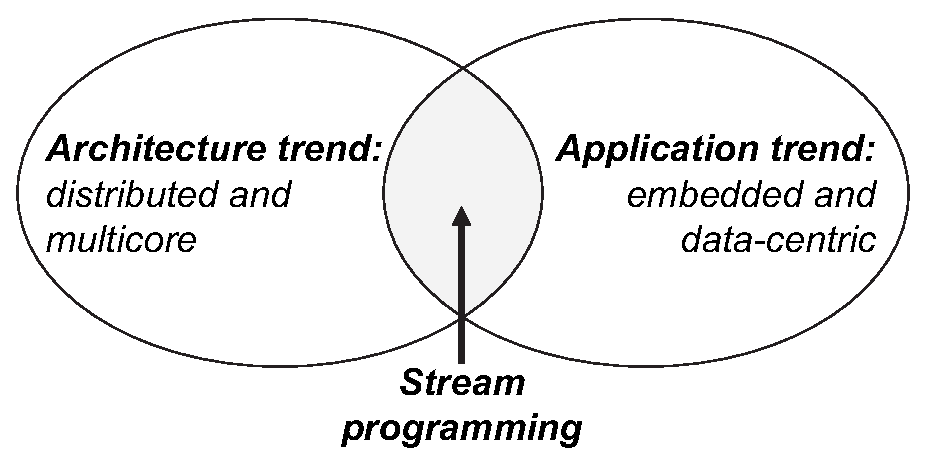
\psfig{file=intersection.eps,width=\myfigwidth}
\end{center}
\vspace{-32pt}
{\mbox{~}\hfill \it \scriptsize Figure inspired by Mattson \& Lethin~\cite{mattson_streaming_2003}}
\vspace{4pt}
\caption[Stream programming is motivated by architecture and
  application trends]{Stream programming is motivated by two prominent
  trends: the trend towards parallel computer architectures, and the
  trend towards embedded, data-centric
  computations.\protect\label{fig:intersection}}
\end{figure}

\begin{figure}[t]
\centering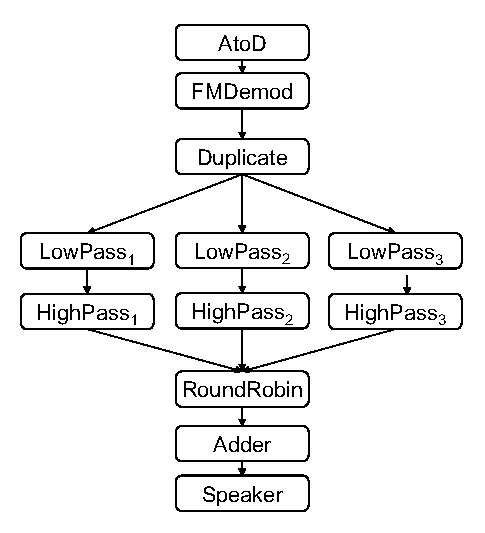
\psfig{file=fm-radio.eps,width=3in}
\caption{Example stream graph for a software radio with equalizer.\protect\label{fig:stream-graph}}
\end{figure}

In this dissertation, we develop language support for stream programs
that enables non-expert programmers to harness both avenues:
parallelism and domain-specific optimizations.  Either set of
optimizations can yield order-of-magnitude performance improvements.
While the techniques used were previously accessible to experts during
manual performance tuning, we provide the first general and automatic
formulation.  This greatly lowers the entry barrier to
high-performance stream programming.

%% In this thesis, we develop language and compiler support for stream
%% programs that enables non-expert programmers to obtain
%% order-of-magnitude performance improvements.  There are two types of
%% improvements: on a multicore architecture, we exploit the parallelism
%% of stream programs to enable robust parallelization in the face of
%% varying application characteristics.  And on a sequential machine, we
%% exploit domain-specific optimizations, including those targetting
%% linear and compressed processing stages.

In the rest of this chapter, we describe the detailed properties of
stream programs, provide a brief history of streaming, give an
overview of the StreamIt project, and state the contributions of this
thesis.

\section{Streaming Application Domain}

Based on the examples cited previously, we have observed that stream
programs share a number of characteristics.  Taken together, they
define our conception of the streaming application domain:

\begin{enumerate}

\item {\it Large streams of data.}  Perhaps the most fundamental
  aspect of a stream program is that it operates on a large (or
  virtually infinite) sequence of data items, hereafter referred to as
  a {\it data stream}.  Data streams generally enter the program from
  some external source, and each data item is processed for a limited
  time before being discarded.  This is in contrast to scientific
  codes, which manipulate a fixed input set with a large degree of
  data reuse.

\item {\it Independent stream filters.}  Conceptually, a streaming
  computation represents a sequence of transformations on the data
  streams in the program.  We will refer to the basic unit of this
  transformation as a {\it filter}: an operation that--on each
  execution step--reads one or more items from an input stream,
  performs some computation, and writes one or more items to an output
  stream.  Filters are generally independent and self-contained,
  without references to global variables or other filters.  A stream
  program is the composition of filters into a {\it stream graph}, in
  which the outputs of some filters are connected to the inputs of
  others.

\item {\it A stable computation pattern.}  The structure of the stream
  graph is generally constant during the steady-state operation of a
  stream program.  That is, a certain set of filters are repeatedly
  applied in a regular, predictable order to produce an output stream
  that is a given function of the input stream.

\item {\it Occasional modification of stream structure.}  Even though
  each arrangement of filters is executed for a long time, there are
  still dynamic modifications to the stream graph that occur on
  occasion.  For instance, if a wireless network interface is
  experiencing high noise on an input channel, it might react by
  adding some filters to clean up the signal; or it might
  re-initialize a sub-graph when the network protocol changes from
  802.11 to Bluetooth\footnote{In this dissertation, we do not explore
    the implications of dynamically modifying the stream structure.
    As detailed in Chapter~2, we operate on a single stream graph at a
    time; users may transition between graphs using wrapper code.}.

%% There is typically an enumerable number of configurations that the
%% stream graph can adopt in any one program, such that all of the
%% possible arrangements of filters are known at compile time.

\item {\it Occasional out-of-stream communication.}  In addition to
  the high-volume data streams passing from one filter to another,
  filters also communicate small amounts of control information on an
  infrequent and irregular basis.  Examples include changing the
  volume on a cell phone, printing an error message to a screen, or
  changing a coefficient in an adaptive FIR filter.  These messages
  are often synchronized with some data in the stream--for instance,
  when a frequency-hopping radio changes frequencies at a specific
  point of the transmission.

\item {\it High performance expectations.}  Often there are real-time
  constraints that must be satisfied by stream programs; thus,
  efficiency (in terms of both latency and throughput) is of primary
  concern.  Additionally, many embedded applications are intended for
  mobile environments where power consumption, memory requirements,
  and code size are also important.

\end{enumerate}

While our discussion thus far has emphasized the embedded context for
streaming applications, the stream abstraction is equally important in
desktop and server-based computing.  Examples include XML
processing~\cite{barton_streaming_2003}, digital filmmaking, cell
phone base stations, and hyperspectral imaging.
% TODO: more examples?

%% As illustrated in Figure~\ref{fig:example-streaming}, these
%% programs can typically be written as a set of independent {\it
%% actors} which communicate over explicit data channels.

\section{Brief History of Streaming}

\begin{figure}[t]
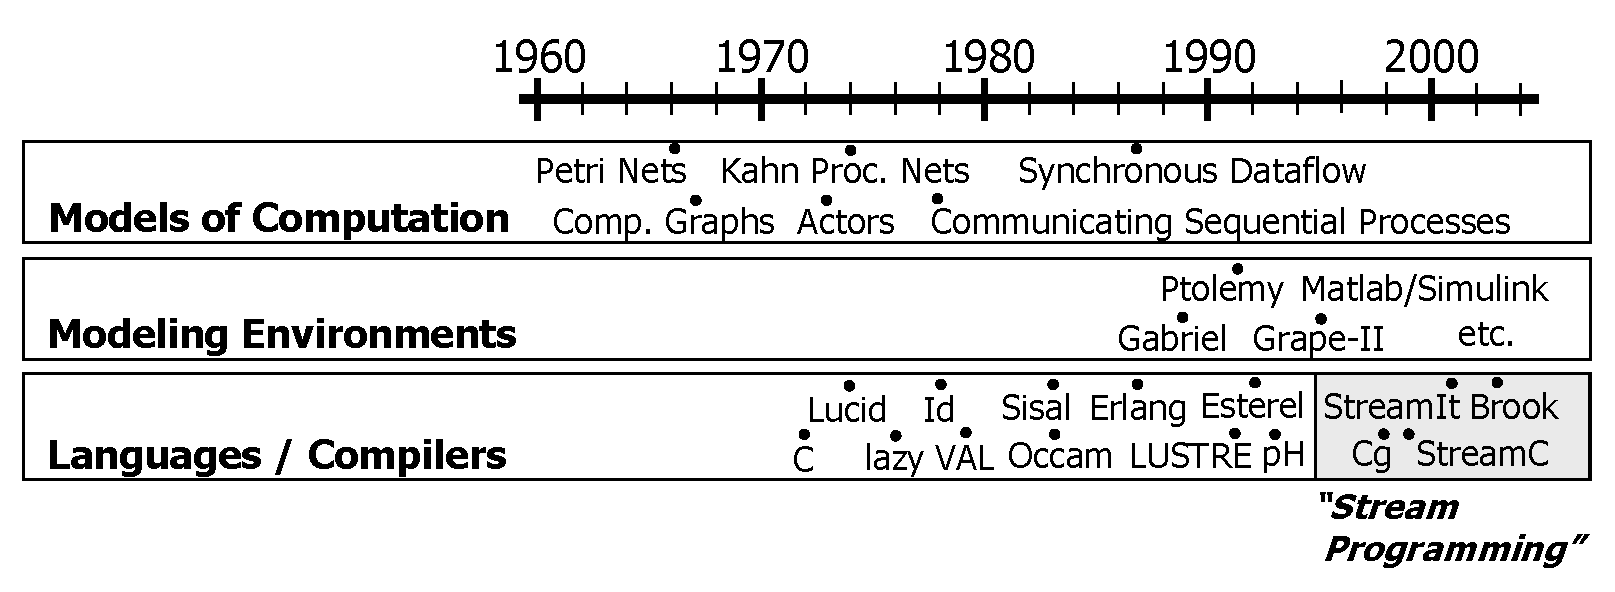
\psfig{file=history-of-streaming.eps,width=\textwidth}
\caption{A timeline of computer science efforts that have incorporated
  notions of streams.\protect\label{fig:history-of-streaming}}
% TODO: note that some dates (lucid?  id?) pulled from Stephens or
% Wikipedia (occam?) for first release
\end{figure}

The concept of a stream has a long history in computer science; see
Stephens~\cite{stephens_survey_1997} for a review of its role in
programming languages.  Figure~\ref{fig:history-of-streaming} depicts
some of the notable events on a timeline, including models of
computation and prototyping environments that relate to streams.

The fundamental properties of streaming systems transcend the details
of any particular language, and have been explored most deeply as
abstract models of computation.  These models can generally be
considered as graphs, where nodes represent units of computation and
edges represent FIFO communication channels.  The models differ in the
regularity and determinism of the communication pattern, as well as
the amount of buffering allowed on the channels.  Three of the most
prevalent models are Kahn Process Networks~\cite{kahn_semantics_1974},
Synchronous Dataflow~\cite{lee_static_1987}, and Communicating
Sequential Processes~\cite{hoare_communicating_1978}.  They are
compared in Figure~\ref{fig:models-of-computation} and
Table~\ref{tab:model-table} and detailed below:

\begin{enumerate}

\item {\it Kahn Process Networks}, also known as {\it process
  networks}, are a simple model in which nodes can always enqueue
  items onto their output channels, but attempts to read from an input
  channel will block until data is ready (it is not possible to test
  for the presence or absence of data on input channels).  Assuming
  that each node performs a deterministic computation, these
  properties imply that the entire network is deterministic; that is,
  the sequence of data items observed on the output channels is a
  deterministic function of those submitted to the input channels.
  However, it is undecidable to statically determine the amount of
  buffering needed on the channels, or to check whether the
  computation might deadlock.  Process networks is the model of
  computation adopted by UNIX pipes.

\item {\it Synchronous Dataflow (SDF)} is a restricted form of process
  network in which nodes execute atomic steps, and the number of data
  items produced and consumed during each step are constant and known
  at compile time.  Because the input and output rates are known, the
  compiler can statically check whether a deadlock-free execution
  exists and, if so, can derive a valid schedule of node executions.
  The amount of buffering needed can also be determined statically.
  Many variations of synchronous dataflow have been defined, including
  cyco-static
  dataflow~\cite{bilsen_cyclo-static_1995,parks_comparison_1995} and
  multidimensional synchronous
  dataflow~\cite{murthy_multidimensional_2002}.  Due to its potential
  for static scheduling and optimization, synchronous dataflow
  provides the starting point for our work.

\begin{figure}[t]
\centering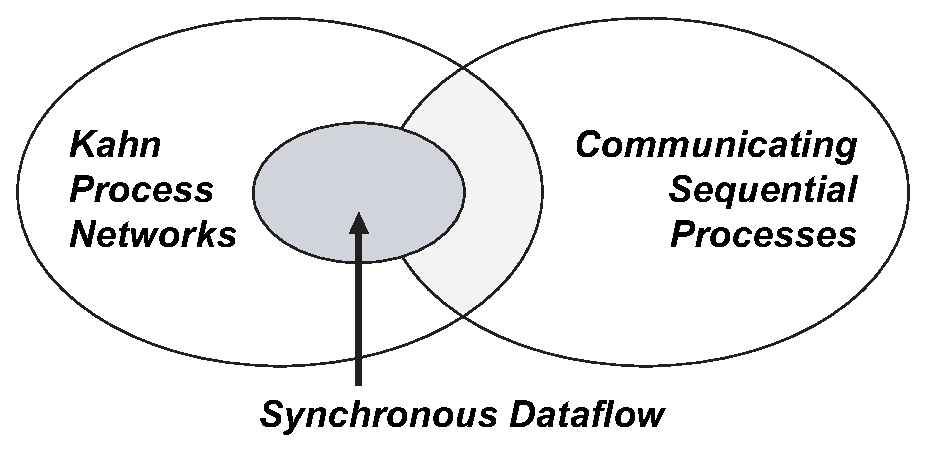
\psfig{file=models-of-computation.eps,width=\myfigwidth}
\caption[Space of behaviors allowable by different models of
  computation]{Space of behaviors allowed by Kahn process networks,
  synchronous dataflow (SDF), and communicating sequential processes
  (CSP).  The set of behaviors considered are: buffering data items on
  a communication channel, making a non-deterministic choice, and
  deviating from a fixed I/O rate.  While these behaviors could always
  be emulated inside a single Turing-complete node, we focus on the
  behavior of the overall graph.
  \protect\label{fig:models-of-computation}}
\end{figure}

\begin{table}[t]
\centering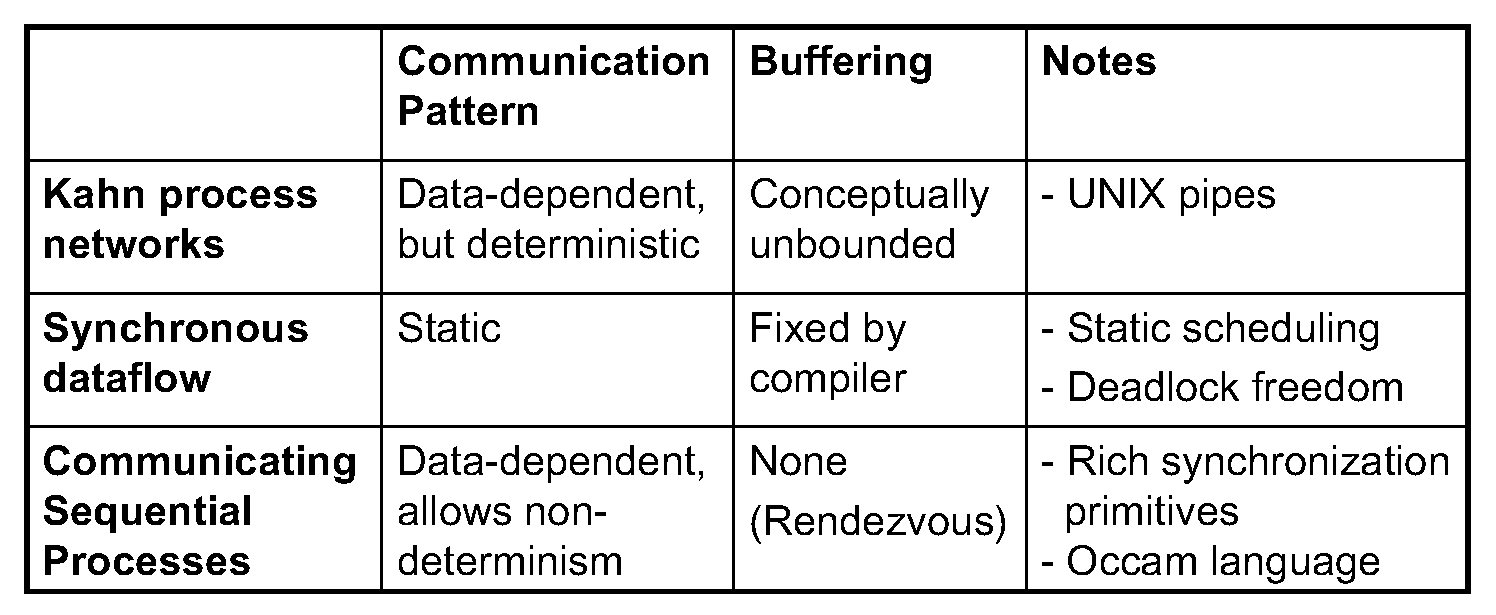
\psfig{file=model-table.eps,width=4.75in}
\caption{Key properties of streaming models of
  computation.\protect\label{tab:model-table}}
\end{table}

\item {\it Communicating Sequential Processes (CSP)} is in some ways
  more restrictive, and in others more flexible than process networks.
  The restriction is rendezvous communication: there is no buffering
  on the communication channels, which means that each send statement
  blocks until being paired with a receive statement (and vice-versa).
  The flexibility is in the synchronization: a node may make a
  non-deterministic choice, for example, in reading from any input
  channel that has data available under the current schedule.  This
  property leads to possibly non-deterministic outputs, and deadlock
  freedom is undecidable.  While CSP itself is an even richer algebra
  for describing the evolution of concurrent systems, this graph-based
  interpretation of its capabilities applies to many of its practical
  instantiations, including the Occam programming language.

\end{enumerate}

While long-running (or infinite) computations are often described
using one of the models above, the descriptions of finite systems also
rely on other models of computation.  {\it Computation
  graphs}~\cite{karp_properties_1966} are a generalization of SDF
graphs; nodes may stipulate that, in order to execute a step, a
threshold number of data items must be available on an input channel
(possibly exceeding the number of items consumed by the node).  While
SDF scheduling results can be adapted to the infinite execution of
computation graphs, the original theory of computation graphs focuses
on determinacy and termination properties when some of the inputs are
finite.  {\it Actors} are a more general model providing asynchronous
and unordered message passing between composable, dynamically-created
nodes~\cite{hewitt_universal_1973,greif_semantics_1975,clinger_foundations_1981,agha_actors:model_1985}.
Petri nets are also a general formalism for modeling many classes of
concurrent transition
systems~\cite{petri_communication_1962,murata_petri_1989}.

In addition to models of computation, prototyping environments have
been influential in the history of streaming systems.  The role of a
prototyping environment is to simulate and validate the design of a
complex system.  While it has been a long-standing goal to
automatically generate efficient and deployable code from the
prototype design, in practice most models are re-written by hand in a
low-level language such as C in order to gain the full performance and
functionality needed.  Still, many graph-level optimizations, such as
% TODO: add more citations, and duplicate below under ``rich, high level analysis''
scheduling~\cite{bhattacharyya_optimal_1995,bhattacharyya_software_1996,bhattacharyya_self-timed_1996,zitzler_multidimensional_2000,stuijk_exploring_2006}
and buffer management~\cite{ad_data_1997,murthy_shared_2001,govindarajan_minimizing_2002,murthy_buffer_2004,geilen_minimising_2005}, have
been pioneered in the context of prototyping environments.  One of the
most long-running efforts is Ptolemy, a rich heterogeneous modeling
environment that supports diverse models of computation, including the
dataflow models described previously as well as continuous- and
discrete-event systems~\cite{buck_multirate_1991,eker_taming_2003}.
Other academic environments include
Gabriel~\cite{lee_gabriel:design_1989},Grape-II~\cite{lauwereins_grape-ii:system-level_1995},
and El Greco~\cite{buck_heterogeneous_2000}, while commercial
environments include MATLAB/Simulink (from The MathWorks, Inc.),
Cocentric System Studio (from Synposis, Inc.), and System Canvas (from
Angeles Design Systems~\cite{murthy_system_2001}).
% TODO: expand list of companies

% True but who cares:
% - first mention of stream by P.J. Landin~\cite{landin_correspondence_1965}
% - lucid originally developed as independent functional language to
%   verify proofs; later seen to be good match for dataflow

The notion of streams has also permeated several programming paradigms
over the past half-century.  Dataflow languages such as
Lucid~\cite{ashcroft_lucidnonprocedural_1977},
Id~\cite{arvind_asynchronous_1978,nikhil_id_1991}, and
VAL~\cite{ackerman_VAL--value-oriented_1979} aim to eliminate
traditional control flow in favor of a scheduler that is driven only
by data dependences.  To expose these dependences, each variable is
assigned only once, and each statement is devoid of non-local side
effects.  These properties overlap streaming in two ways.  First, the
producer/consumer relationships exposed by dataflow are similar to
those in a stream graph, except at a much finer level of granularity.
Second, to preserve the single-assignment property within loops, these
languages use a {\it next} keyword to indicate the value of a variable
in the succeeding iteration.  This construct can be viewed as a
regular data stream of values flowing through the loop.  Subsequent
dataflow languages include Sisal~\cite{mcgraw_sisal:_1985} (``streams
and iteration in a single assignment language'')
% True but who cares:
%, which grew out of VAL,
and pH~\cite{nikhil_implicit_2001}.
% True but who cares:
%, which grew out of  grew out of Id and Sisal.
More details on dataflow languages available in review
articles~\cite{johnston_advances_2004,stephens_survey_1997}.

Functional languages also have notions of streams, for example, as
part of the lazy evaluation of lists~\cite{henderson_lazy_1976}.  It
bears noting that seems to be no fundamental difference between a
``functional language'' and a ``dataflow language''.  The terminology
indicates mainly a difference of community, as dataflow languages were
mapped to dataflow machines.  In addition, dataflow languages may be
more inclined toward an imperative
syntax~\cite{johnston_advances_2004}.  We do not survey functional
languages further in their own right.

Another class of languages is synchronous languages, which offer the
abstraction of responding instantly (in synchrony) with their
environment~\cite{halbwachs_synchronous_1998}.  Interpreted as a
stream graph, a synchronous program can be thought of as a circuit,
where nodes are state machines and edges are wires that carry a single
value; in some languages, nodes may specify the logical times at which
values are present on the wires.  Synchronous programs target the
class of reactive systems, such as control circuits, embedded devices,
and communication protocols, where the computation is akin to a
complex automaton that continually responds to real-time events.
Compared to stream programs, which have regular, computation-intensive
processing, synchronous programs process irregular events and demand
complex control flow.  Key synchronous languages include
Signal~\cite{le_guernic_signal--data_1986},
LUSTRE~\cite{caspi_lustre:declarative_1987,halbwachs_synchronous_1991},
Esterel~\cite{berry_esterel_1992}, and
Argos~\cite{maraninchi_argos:automaton-based_2001}.  These languages offer
determinism and safety properties, spurring their adoption in
industry; Esterel Technologies offers SCADE (based on LUSTRE) as well
as Esterel Studio.

There have also been general-purpose languages with built-in support
for streams, including Occam~\cite{occammanual} and
Erlang~\cite{armstrong_concurrent_1993,armstrong_history_2007}.  Occam
is an imperative procedural language that is based on communicating
sequential processes; it was originally developed to for the INMOS
transputer, an early multiprocessor.  Erlang is a functional language
that is based on the actors model; originally developed by Ericsson
for distributed applications, it supports very lightweight processes
and has found broad application in industry.

{\bf Shortcomings of previous languages.}  It should be evident that
previous languages have provided many variations on streams, including
many elegant and general ways of expressing the functional essence of
streaming computations.  However, there remains a critical disconnect
in the design flow for streaming systems: while prototyping
environments provide rich, high-level analysis and optimization of
stream
graphs~\cite{bhattacharyya_optimal_1995,bhattacharyya_software_1996,bhattacharyya_self-timed_1996,ad_data_1997,zitzler_multidimensional_2000,murthy_shared_2001,govindarajan_minimizing_2002,murthy_buffer_2004,geilen_minimising_2005,stuijk_exploring_2006},
these optimizations have not been automated in any programming
language environment and thus remain out-of-reach for the vast
majority of developers.  The root of the disconnect is the model of
computation: previous languages have opted for the flexibility of
process networks or communication sequential processes, rather than
embracing the restrictive yet widely-applicable model of synchronous
dataflow.  By focusing attention on a very common case -- an
unchanging stream graph with fixed communication rates -- synchronous
dataflow is the only model of computation that exposes the information
needed to perform static scheduling and optimization.

Herein lies a unique opportunity to create a language that exposes the
inherent regularity in stream programs, and to exploit that regularity
to perform deep optimizations.  This is the opportunity that we pursue
in the StreamIt project.

%% This idea is at the core of the movement known as {\it stream
%%   programming}, which encompasses related efforts such as
%% Cg~\cite{mark_cg:system_2003},
%% StreamC~\cite{TODO-might-have-to-change-date-in-figure}, and
%% Brook~\cite{buck_brook_2004}.  Our work on the StreamIt project was
%% one of the early efforts in this space.

\section{The StreamIt Project}

StreamIt is a language and compiler for high-performance stream
programs.  The principal goals of the StreamIt project are three-fold:

\begin{enumerate}

\item To expose and exploit the inherent parallelism in stream
  programs on multicore architectures.

\item To automate domain-specific optimizations known to streaming
  application specialists.

\item To improve programmer productivity in the streaming domain.

\end{enumerate}

While the first two goals are related to performance improvements, the
third relates to improving programmability.  We contend that these
goals are not in conflict, as high-level programming models contain
more information and can be easier to optimize while also being easier
to use.  However, many languages are designed only from the standpoint
of programmability, and often make needless sacrifices in terms of
analyzability.  Compared to previous efforts, the key leverage of the
StreamIt project is a {\it compiler-conscious language design} that
maximizes both analyzability and programmability.

% People mentioned:
%% Ali Meli
%% Andrew Lamb
%% Basier Aziz
%% Bill Thies
%% Chris Leger
%% Ceryen Tan
%% David Zhang
%% Hank Hoffmann
%% Janis Sermulins
%% Jeremy Wong
%% Jiawen Chen
%% Kimberly Kuo
%% Kunal Agrawal
%% Mani Narayanan
%% Matt Brown
%% Matthew Drake
%% Michael Gordon
%% Michal Karczmarek
%% Phil Sung
%% Qiuyuan Li
%% Rodric Rabbah
%% Saman Amarasinghe
%% Satish Ramaswamy
%% Shirely Fung
%% Sitij Agrawal
%% Steve Hall
%% Weng-Fai Wong

StreamIt is a large systems project, incorporating over 27 people (up
to 12 at a given time).  The group has made several contributions to
the goals highlighted above.  In exploiting parallelism, Michael
Gordon led the development of the first general algorithm that
exploits the task, data, and pipeline parallelism in stream
programs~\cite{gordon-asplos06}.  On the 16-core Raw architecture, it
achieves an 11x mean speedup for our benchmark suite; this is a 1.8x
improvement over our previous
approach~\cite{gordon-asplos02,gordon-thesis}, the performance of
which had been modeled by Jeremy Wong~\cite{wong-thesis}.  Also on the
Raw machine, Jiawen Chen led the development of a flexible graphics
rendering pipeline in StreamIt, demonstrating that a reconfigurable
pipeline can achieve up to twice the throughput of a
static~\cite{chen-graphics05,chen_load-balanced_2005}.  Moving beyond
Raw, Janis Sermulins ported StreamIt to multicores and clusters of
workstations, and also led the development of cache optimizations that
offer a 3.5x improvement over unoptimized StreamIt on embedded
processors~\cite{sermulins-lctes05,sermulins-thesis}.  David Zhang and
Qiuyuan Li led the development of a flexible streaming execution layer
that achieves over 88\% utilization on the Cell
processor~\cite{zhang_lightweight_2007,zhang-thesis}.  Michal
Karczmarek led the development of phased scheduling, the first
hierarchical scheduler for cyclo-static dataflow that also enables a
flexible tradeoff between code size and buffer
size~\cite{karczmarek-lctes03,karczmarek-thesis}.  Phil Sung and
Weng-Fai wong explored the execution of StreamIt on graphics
processors.

%- appears in the evaluation of the Raw architecture~\cite{taylor2004}

In the area of domain-specific optimizations, Andrew Lamb automated
the optimization of linear nodes, performing coarse-grained algebraic
simplification or automatic conversion to the frequency
domain~\cite{lamb-pldi03,lamb-thesis}.  These inter-node
optimizations eliminate 85\% of the floating point operations from
code written in a modular style.  Sitij Agrawal generalized the
analysis to handle linear computations with state, performing
optimizations such as algebraic simplification, removal of redundant
states, and reducing the number of
parameters~\cite{agrawal-cases05,agrawal-thesis}.  I led the
development of domain-specific optimizations for compressed data
formats, allowing certain computations to operate in place on the
compressed data without requiring decompression and
re-compression~\cite{thies-compression07}.  This transformation
accelerates lossless video editing operations by a median of 15x.

In the area of programmability, we as a group defined the StreamIt
language, incorporating the first notions of structured, hierarchical
streams as well as language support for reordering and sliding-window
operations~\cite{thies-cc02,thies-can02,amarasinghe-ijpp05}.  With
Michal Karczmarek and Janis Sermulins, I led the development of
teleport messaging, a new language construct that uses the flow of
data in the stream to provide a deterministic and meaningful timeframe
for delivering events between decoupled nodes~\cite{thies-ppopp05}.
Kimberly Kuo developed an Eclipse development environment and debugger
for StreamIt and, with Rodric Rabbah, demonstrated improved
programming outcomes in a user study~\cite{kuo05,kuo-thesis}.
Juan Reyes also developed a graphical editor for
StreamIt~\cite{reyes-thesis}.  Matthew Drake evaluated StreamIt's
suitability for video codecs by implementing an MPEG-2 encoder and
decoder~\cite{drake-ipdps06,drake-thesis}.  Basier Aziz evaluated
StreamIt by implementing image-based motion estimation, including the
RANSAC algorithm~\cite{aziz-thesis}.  I also led the development of
dynamic analysis tools to ease the translation of legacy C code into a
streaming representation~\cite{thies-micro07}.

The StreamIt benchmark suite has been used by outside
researchers~\cite{kudlur_orchestratingexecution_2008}.
% TODO: add more users of benchmarks?
In addition to MPEG-2 and image-based motion estimation, the
60,000-line suite includes a ground moving target indicator (GMTI), a
feature-aided tracker (FAT), synthetic aperture radar (SAR), a radar
array front-end, part of the 3GPP physical layer, a vocoder with
speech transformation, a subset of an MP3 decoder, a subset of MPEG-4
decoder, a JPEG encoder and decoder, a GSM decoder, an FM software
radio, DES and serpent encryption, matrix multiplication, graphics
shaders and rendering algorithms, and various DCTs, FFTs, filterbanks,
and sorting algorithms.  Some programs are currently restricted for
internal use.
% TODO: Fix order?
Contributors to the benchmark suite include Sitij Agrawal, Saman
Amarasinghe, Basier Aziz, Matt Brown, Jiawen Chen, Matthew Drake,
Shirley Fung, Michael Gordon, Hank Hoffmann, Michal Karczmarek, Andrew
Lamb, Chris Leger, Ali Meli, Mani Narayanan, Rodric Rabbah, Satish
Ramaswamy, and Jeremy Wong.

%% includes GMTI radar processing (by Sitij Agrawal), part of the 3GPP
%% physical layer (by Ali Meli), a vocoder (by Chris Leger), a subset
%% of MP3 decoding (by Michal Karczmarek), a GSM decoder (by Jeremy
%% Wong), an FM software radio (by Matt Brown), various FFTs (by
%% Michal Karczmarek, Satish Ramaswamy, and Mani Narayanan) and
%% various sorting algorithms (by Chris Leger and Mani Narayanan).

While this section was not intended to serve as the acknowledgments,
it would be incomplete without noting the deep involvement, guidance,
and supervision of Rodric Rabbah and Saman Amarasinghe throughout many
of the efforts listed above.  The StreamIt infrastructure was also
made possible by the tenacious and tireless efforts of David Maze,
Jasper Lin, and Allyn Dimock.  Additional contributors that were not
mentioned previously include Kunal Agrawal (who developed bit-level
analyses), Steve Hall (who automated compressed-domain
transformations), and Ceryen Tan (who is improving the multicore
backend).

The StreamIt compiler (targeting shared-memory multicores, clusters of
workstations, and the MIT Raw machine) is publicly
available~\cite{streamitweb} and has logged over 700 unique,
registered downloads from 225 institutions.  Researchers at other
universities have used StreamIt as a basis for their own
work~\cite{mani-permutations,bit-streaming,ola-techrep,duca-thesis,won-thesis}.

This dissertation does not mark the culmination of the StreamIt
project; please consult the StreamIt website~\cite{streamitweb} for
subsequent updates.

\section{Contributions}

My role in the StreamIt project has been very collaborative,
contributing ideas and implementation support to many aspects of the
project.  This dissertation focuses on ideas that have not been
presented previously in theses by other group members.  However, to
provide a self-contained view of the breadth and applications of
StreamIt, Chapter~\cite{chap:optimizing} also provides a survey of
others' experience in optimizing the language.

The specific contributions of this dissertation are as follows:

\begin{enumerate}

\item {\it A design rationale and experience report for the StreamIt
  language, which contains novel constructs to simultaneously improve
  the programmability and analyzability of stream programs
  (Chapter~2).}  StreamIt is the first language to introduce
  structured streams, as well as hierarchical, parameterized data
  reordering.  We also describe the lessons learned in developing the
  60,000-line StreamIt benchmark suite.

\item {\it A new language construct, termed teleport messaging, that
  enables precise event handling in a distributed environment
  (Chapter~3).}  Teleport messaging is a general approach that uses
  the flow of data in the stream to provide a deterministic and
  meaningful timeframe for delivering events between decoupled nodes.
%  We formulate a stream dependence function, {\sdep}, which provides
%  the first coordinated timeframe between distributed actors.
  Teleport messaging allows irregular control messages to be
  integrated into a synchronous dataflow program while preserving
  static scheduling.

\item {\it A review of the key results in optimizing StreamIt,
  spanning parallelization and domain-specific optimization
  (Chapter~4)}.  This chapter validates key concepts of the StreamIt
  language by highlighting the gains in performance and
  programmability that have been achieved, largely due to the work of
  others in the StreamIt group.  We focus on automatic parallelization
  (providing an 11.6x speedup on a 16-core machine), domain-specific
  optimization of linear computations (eliminating up to 85\% of the
  floating point operations), and cache optimizations (providing a
  3.5x speedup on embedded processors).

\item {\it The first translation of stream programs into the
  lossless-compressed domain (Chapter~5)}.  This domain-specific
  optimization allows stream programs to operate directly on
  compressed data formats, rather than requiring conversion to an
  uncompressed format prior to processing.  While previous researchers
  have focused on compressed-domain techniques for lossy data formats,
  there are few techniques that apply to lossless formats.  We focus
  on applications in video editing, where our technique supports color
  adjustment, video compositing, and other operations directly on the
  Apple Animation format (a variant of LZ77).  Speedups are roughly
  proportional to the compression factor, with a median of 15x.

\item {\it The first dynamic analysis tool that detects and exploits
  likely coarse-grained parallelism in C programs (Chapter~6).}  To
  assist programmers in migrating legacy C code into a streaming
  representation, this tool generates a stream graph depicting dynamic
  communication between programmer-annotated sections of code.  The
  tool can also generate a parallel version of the program based on
  the memory dependences observed during training runs.  In our
  experience with six case studies, the extracted stream graphs prove
  useful and the parallelized versions offer a 2.78x speedup on a
  4-core machine.

\end{enumerate}

% support claim of order-of-magnitude

\noindent Lessons learned and future work are described in the
conclusion (Chapter~7).

\newpage

Alternate opening paragraph:
\medskip

While the advent of high-level programming languages has made it
easier for beginner programmers to construct working applications,
optimizing the performance of those applications is a more difficult
task that is often beyond the reach of non-experts.  To improve the
execution time, a performance expert may re-write large sections of
the application, employing alternative algorithms, data structures, or
task decompositions, to produce a version that is functionally
equivalent to (but structurally very different from) the original
program.  They may also utilize in-depth knowledge of the target
architecture, such as the type and extent of parallel resources, the
communication substrate, and the cache sizes, to match the structure
and granularity of the application to that of the underlying machine.
While it has been a long-term goal of the computer science community
to replicate the role of performance experts via systematic
transformations within the compiler, many optimizations remain beyond
the reach of automation because the compiler does not have the
information needed -- either about the program itself, or about the
class of transformations known to the expert -- to match the
hand-tuned performance.
